We used a cycle-GAN
\footnote{\url{https://github.com/junyanz/pytorch-CycleGAN-and-pix2pix/}}.
With a limited selection of pre-trained models, we used a pretrained photo to Van Gogh network.
These classes proved poor approximations of games and movies and this model didn't achieve the desired style.
Instead we trained 2 background models, one from scratch and one extending the photo2vangogh model.
The model from scratch preformed best, so after applying data augmentations we retrained the network from scratch giving some good results \ref{fig:Q2_1}.
We note that while training we experienced mode collapse, across training epoch game outputs cycle between being having a green and brown tinges.

\begin{figure}[h!]
  \begin{center}
  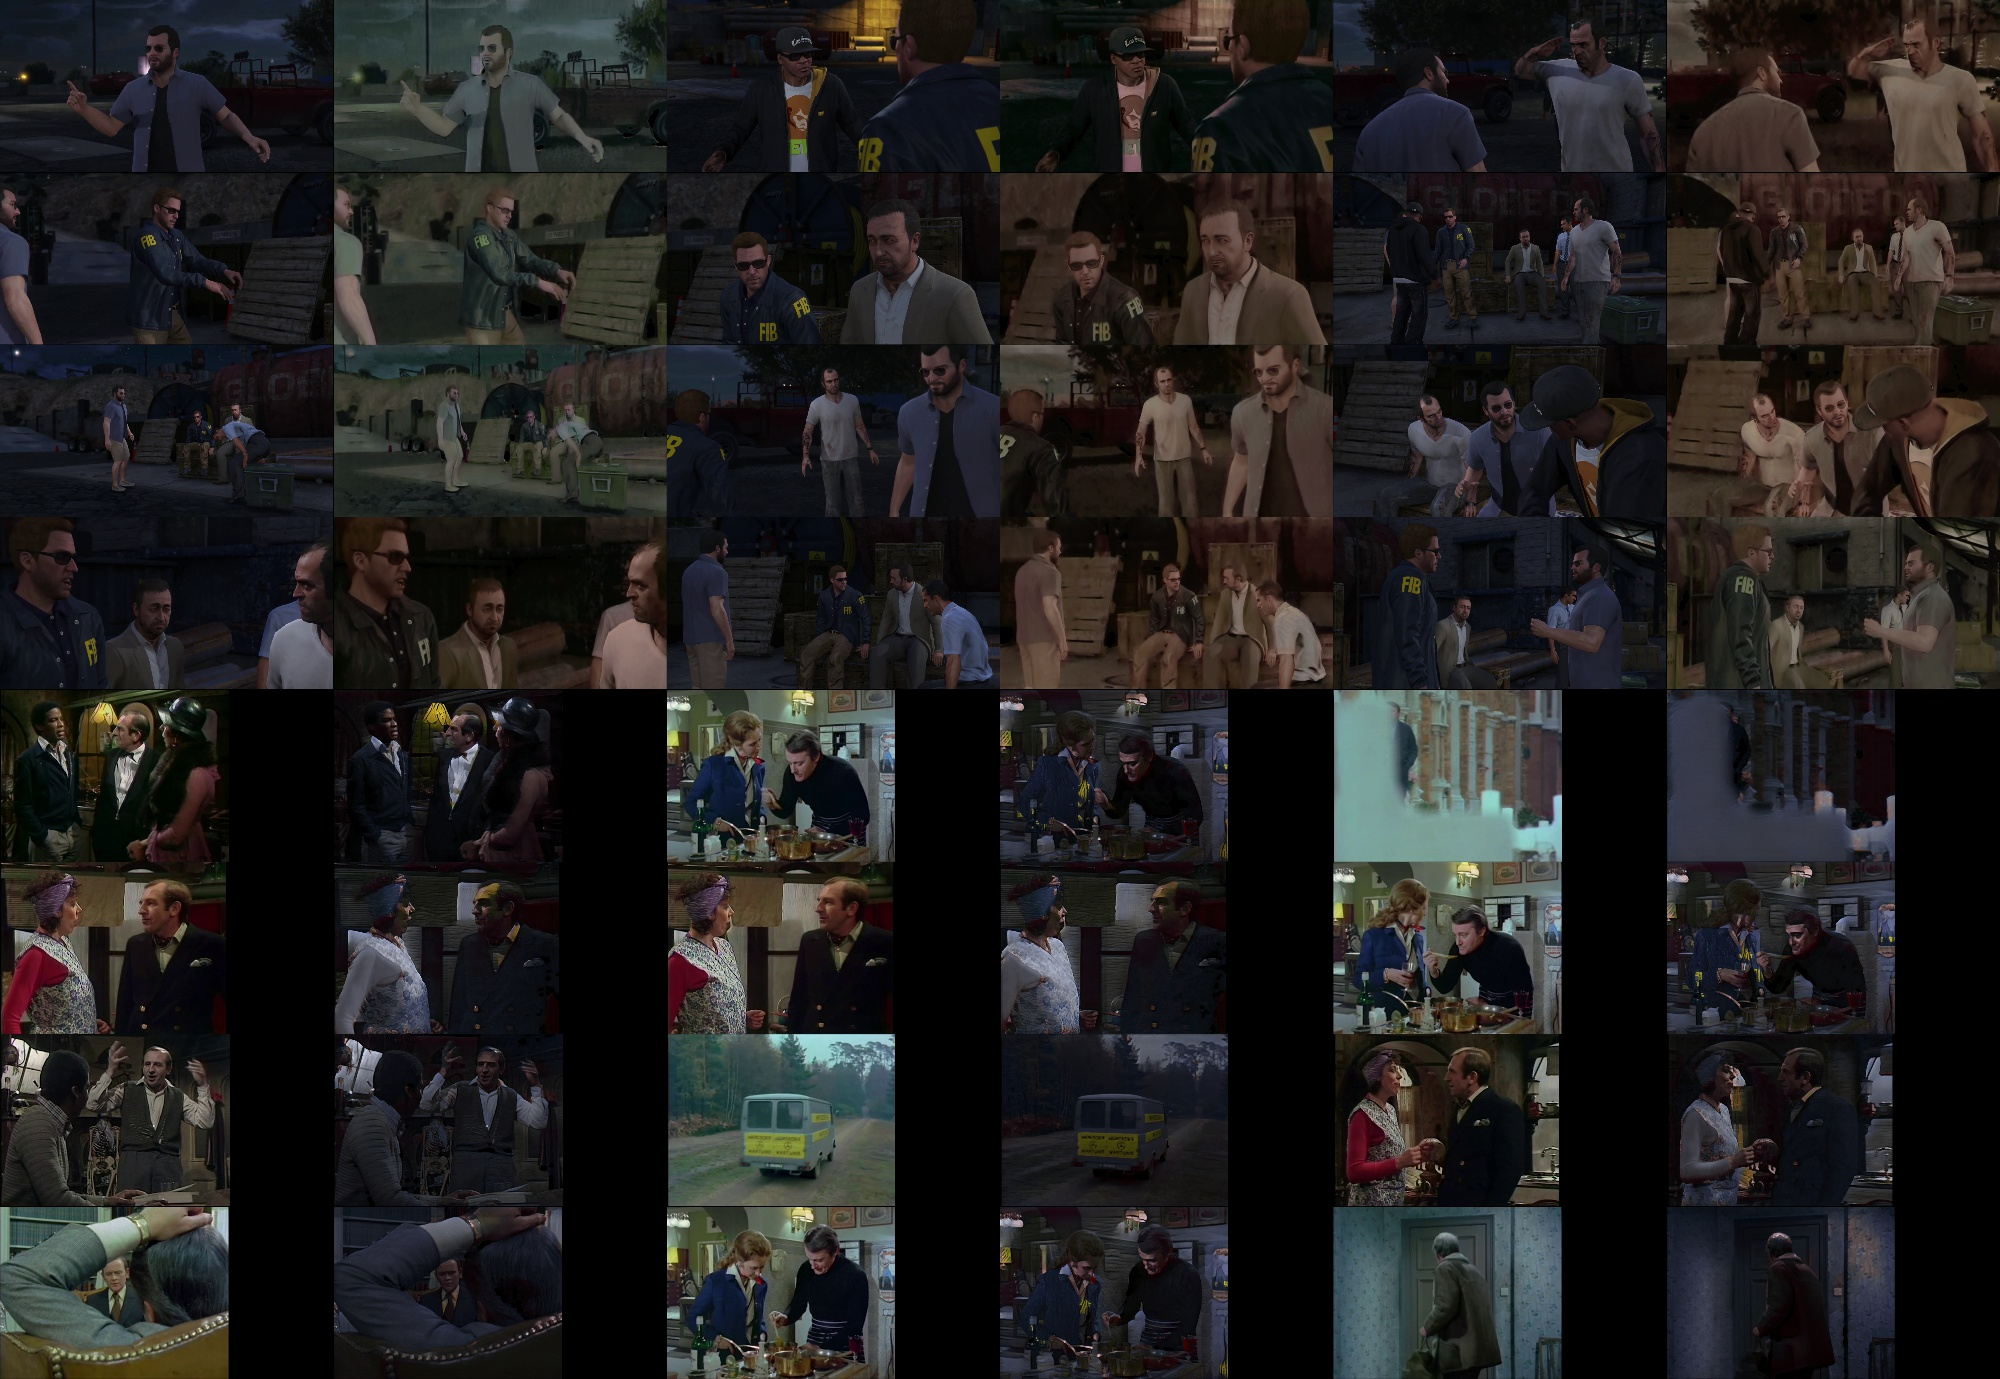
\includegraphics[scale=0.2]{Q2_1_25.jpg}
    \caption{Q2.1 sample of background frames (left) and style transfer into other domain (right).}
    \label{fig:Q2_1}
  \end{center}
  \end{figure}